\documentclass[10pt,article,oneside]{memoir}
\usepackage{lmodern}
\usepackage{amssymb,amsmath}
\usepackage{ifxetex,ifluatex}
\usepackage{fixltx2e} % provides \textsubscript
\ifnum 0\ifxetex 1\fi\ifluatex 1\fi=0 % if pdftex
  \usepackage[T1]{fontenc}
  \usepackage[utf8]{inputenc}
\else % if luatex or xelatex
  \ifxetex
    \usepackage{mathspec}
    \usepackage{xltxtra,xunicode}
  \else
    \usepackage{fontspec}
  \fi
  \defaultfontfeatures{Mapping=tex-text,Scale=MatchLowercase}
  \newcommand{\euro}{€}
\fi
% use upquote if available, for straight quotes in verbatim environments
\IfFileExists{upquote.sty}{\usepackage{upquote}}{}
% use microtype if available
\IfFileExists{microtype.sty}{%
\usepackage{microtype}
\UseMicrotypeSet[protrusion]{basicmath} % disable protrusion for tt fonts
}{}
\ifxetex
  \usepackage[setpagesize=false, % page size defined by xetex
              unicode=false, % unicode breaks when used with xetex
              xetex]{hyperref}
\else
  \usepackage[unicode=true]{hyperref}
\fi
\hypersetup{breaklinks=true,
            bookmarks=true,
            pdfauthor={},
            pdftitle={HIVE Year 1 Report: Executive Summary},
            colorlinks=true,
            citecolor=blue,
            urlcolor=blue,
            linkcolor=magenta,
            pdfborder={0 0 0}}
\urlstyle{same}  % don't use monospace font for urls
\usepackage{fancyhdr}
\pagestyle{fancy}
\pagenumbering{arabic}
\lhead{\itshape A Commodity Performance Baseline for HIVE Graph Applications:\\Year 1 Report}
\chead{}
\rhead{\itshape{\nouppercase{\leftmark}}}
% \lfoot{v }
% \lfoot{}
\cfoot{\thepage}
% \rfoot{\thepage}
\usepackage{longtable,booktabs}
\usepackage{graphicx,grffile}
\makeatletter
\def\maxwidth{\ifdim\Gin@nat@width>\linewidth\linewidth\else\Gin@nat@width\fi}
\def\maxheight{\ifdim\Gin@nat@height>\textheight\textheight\else\Gin@nat@height\fi}
\makeatother
% Scale images if necessary, so that they will not overflow the page
% margins by default, and it is still possible to overwrite the defaults
% using explicit options in \includegraphics[width, height, ...]{}
\setkeys{Gin}{width=\maxwidth,height=\maxheight,keepaspectratio}
\setlength{\parindent}{0pt}
\setlength{\parskip}{6pt plus 2pt minus 1pt}
\setlength{\emergencystretch}{3em}  % prevent overfull lines
\providecommand{\tightlist}{%
  \setlength{\itemsep}{0pt}\setlength{\parskip}{0pt}}
\setcounter{secnumdepth}{0}

\title{A Commodity Performance Baseline for HIVE Graph Applications:\\Year 1 Report}
\author{Ben Johnson \and Weitang Liu \and Agnieszka Łupińska \and Muhammad Osama \and John D. Owens \and Yuechao Pan \and Leyuan Wang \and Xiaoyun Wang \and Carl Yang}
\postauthor{\end{tabular}\par UC Davis\end{center}}
\date{}

% Redefines (sub)paragraphs to behave more like sections
\ifx\paragraph\undefined\else
\let\oldparagraph\paragraph
\renewcommand{\paragraph}[1]{\oldparagraph{#1}\mbox{}}
\fi
\ifx\subparagraph\undefined\else
\let\oldsubparagraph\subparagraph
\renewcommand{\subparagraph}[1]{\oldsubparagraph{#1}\mbox{}}
\fi

\begin{document}
\maketitle

{
\hypersetup{linkcolor=black}
\setcounter{tocdepth}{0}
\tableofcontents
}
\chapter{Executive Summary}\label{executive-summary}

Herein UC Davis produces the following three deliverables that it
promised to deliver in Year 1:

\begin{enumerate}
\def\labelenumi{\arabic{enumi}.}
\itemsep1pt\parskip0pt\parsep0pt
\item
  \textbf{7--9 kernels running on a single GPU on DGX-1}. The PM had
  indicated that the application targets are the graph-specific kernels
  of larger applications, and that our effort should target these
  kernels. These kernels run on one GPU of the DGX-1. These kernels are
  in Gunrock's GitHub repository as standalone kernels. While we
  committed to delivering 7--9 kernels, we deliver all 11 v0 kernels.
\item
  \textbf{(High-level) performance analysis of these kernels}. In this
  report we analyze the performance of these kernels.
\item
  \textbf{Separable communication benchmark predicting latency and
  throughput for a multi-GPU implementation}. This report (and
  associated code, also in the Gunrock GitHub repository) analyzes the
  DGX-1's communication capabilities and projects how single-GPU
  benchmarks will scale on this machine to 8 GPUs.
\end{enumerate}

\chapter{Geolocation}\label{geolocation}

Infers user locations using the location (latitude, longitude) of
friends through spatial label propagation. Given a graph \texttt{G},
geolocation examines each vertex \texttt{v}`s neighbors and computes the
spatial median of neighbors' location list, the output is a list of
predicted locations for all vertices with unknown locations.

\section{Summary of Results}\label{summary-of-results}

One or two sentences that summarize ``if you had one or two sentences to
sum up your whole effort, what would you say''. I will copy this
directly to the high-level executive summary in the first page of the
report. Talk to JDO about this. Write it last, probably.

\section{Summary of Gunrock
Implementation}\label{summary-of-gunrock-implementation}

We implemented Geolocation using two \texttt{compute} operators as
\texttt{ForAll()}. The first \texttt{ForAll()} is a \texttt{gather}
operation, gathering all the values of neighbors with known locations
for an active vertex \texttt{v}, and the second \texttt{ForAll()} uses
those values to compute the \texttt{spatial\_center} where the spatial
center of a list points is the center of those points on earth's
surface.

See \texttt{gunrock/app/geo/geo\_spatial.cuh} for details on the spatial
center implementation.

\section{How To Run This Application on DARPA's
DGX-1}\label{how-to-run-this-application-on-darpas-dgx-1}

\subsection{Prerequisites}\label{prerequisites}

\subsection{HIVE Data Preparation}\label{hive-data-preparation}

Prepare the data, skip this step if you are just running the sample
dataset. Assuming we are in \texttt{tests/geo} directory:

This will generate two files: \texttt{instagram.mtx} and
\texttt{instagram.labels}, which can be used as an input to the
geolocation app.

\subsection{Running the application}\label{running-the-application}

Application specific parameters:

Example command-line:

Sample input (labels):

Sample output:

\subsection{Output}\label{output}

When \texttt{quick} mode is disabled, the application performs the CPU
Reference implementation, which is used to validate the results from the
GPU implementation. Geolocation application also supports the
\texttt{quiet} mode, which allows user to skip the output and just
report the performance metrics (note, this will run CPU implementation
in the background without any output).

\section{Performance and Analysis}\label{performance-and-analysis}

Runtime is the key metric for measuring performance for Geolocation. We
also check for prediction accuracy of the labels, but that is a
threshold for correctness. If a certain threshold is not met (while
comparing results to the CPU reference code), the output is considered
incorrect and that run is invalid. Therefore, for the report I will just
be focusing on runtime.

\subsection{Implementation
limitations}\label{implementation-limitations}

One of the biggest limitation is that we are currently using
\texttt{\textbar{}V\textbar{}x\textbar{}V\textbar{}} to store all the
neighbors locations for all the vertices. For a graph of size
\texttt{60K} nodes, it can take approximately \texttt{16GB} of a GPU
memory. In the worst case scenario, we have a fully connected graph, but
in most real world we won't see this connectivity within a network. Some
tricks can be done to determine the degree of each vertex before hand
and allocate just enough memory required to store the locations of valid
neighbors. For the sake of complexity and time, we currently using
\texttt{\textbar{}V\textbar{}x\textbar{}V\textbar{}} size array.

\subsection{{[}Optimization{]} Reducing Memory
footprint}\label{optimization-reducing-memory-footprint}

In the new version of Geolocation, we aim to address the memory
limitations of the problem, where \texttt{locations\_list} array being
\texttt{\textbar{}V\textbar{}x\textbar{}V\textbar{}} is not a viable
size GPUs can handle for larger dataset. Devised solution is that the
\texttt{gather} and \texttt{spatial\_center} operators are fused
together such that now there are few more gathers within the spatial
median calculations. Instead of storing the locations in a huge
locations array, they are now fetch as needed within the
\texttt{spatial\_center} operator. Now, the largest allocated array size
is of \texttt{\textbar{}E\textbar{}}, which is way more viable than a
\texttt{\textbar{}V\textbar{}x\textbar{}V\textbar{}}.

\subsection{Comparison against existing
implementations}\label{comparison-against-existing-implementations}

\begin{longtable}[c]{@{}lllllll@{}}
\toprule
Dataset & {[}V{]} & {[}E{]} & Iterations & GT CPU (8 threads) & GT CPU
(serial) & Gunrock\tabularnewline
\midrule
\endhead
geolocation-sample & 39 & 170 & 3 & 0.466108 & N/A &
0.286102\tabularnewline
instagram & 23731995 & 41355870 & 3 & 10.643214 & 63.821812 &
1.910632\tabularnewline
\bottomrule
\end{longtable}

On a GPU filling workload, gunrock out performs GT's C++ implementation
using OpenMP by 5.5x. There is a lack of available dataset to test the
performance against, so we are restricted to only using the provided
instagram dataset, and a toy sample for sanity check. All tested
implementations meet the criteria of accuracy, which is compared against
the output of the original python implementation.

\begin{itemize}
\itemsep1pt\parskip0pt\parsep0pt
\item
  \href{https://gitlab.hiveprogram.com/ggillary/geotagging.git}{HIVE
  reference implementation}
\item
  \href{https://gitlab.hiveprogram.com/gtusc/geotagging}{GTUSC
  implementation}
\end{itemize}

\subsection{Performance limitations}\label{performance-limitations}

As discussed later in the ``Alternate approaches'' section, current
implementation of geolocation uses a compute operator with minimum load
balancing. In cases where the graph is not so nicely distributed (where
there is a great deal of difference in degrees of vertices), the entire
application will suffer significantly from load imbalance.

Profiling the application shows 98.78\% of the compute time in GPU
activities is the \texttt{spatial\_median} kernel, which gives us a good
direction to focus our efforts on load balancing the workloads within
the operator. Specifically, the for loops iterating over the neighbor
list for spatial center calculations.

\section{Next Steps}\label{next-steps}

\subsection{Alternate approaches}\label{alternate-approaches}

\begin{itemize}
\item
  \textbf{Neighborhood Reduce w/ Spatial Center:} We can perform better
  load balancing by opting in for neighbor reduce (\texttt{advance}
  operator + \texttt{cub::DeviceSegmentedReduce}) instead of using a
  compute operator. In graphs where the degree of a nodes could vary a
  lot, the compute operator will significantly be slower than a load
  balanced advance + segmented reduce.
\item
  \textbf{Push Based Approach:} Instead of gathering all the locations
  from all the neighbors of an active vertex, we perform a scatter of
  valid locations of all active vertices to their neighbors; push
  vs.~pull approach.
\end{itemize}

\subsection{Gunrock implications}\label{gunrock-implications}

\begin{itemize}
\itemsep1pt\parskip0pt\parsep0pt
\item
  \textbf{The \texttt{predicted} atomic:} Geolocation and some other
  application exhibit the same behavior where the stop condition of the
  algorithm is such that when all vertices' label is predicted or
  determined, the algorithm stops. In Geolocation's case, when a
  location for all nodes is predicted, geolocation converges. This is
  currently being done with a loop and an atomic and it needs to be more
  of a core operation (mini-operator) such that when
  \texttt{isValidCount(labels\textbar{}V\textbar{})\ ==\ \textbar{}V\textbar{})}
  stop condition is met. Currently, I am skipping this using number of
  iterations parameter to determine how long geolocation should run for.
\end{itemize}

\subsection{Notes on multi-GPU
parallelization}\label{notes-on-multi-gpu-parallelization}

No complicated partitioning scheme is required for multi-GPU
implementation; the challenging part for a multi-GPU Geolocation would
be to obtain the updated node location from a seperate device if the two
vertices on different devices share an edge. An interesting approach
here would be leveraging the P2P memory bandwidth with the new NVLink
connectors to exchange small amount of updates across the NVLink's
memory lane.

\subsection{Notes on dynamic graphs}\label{notes-on-dynamic-graphs}

Streaming graphs is an interesting problem for Geolocation application,
because when predicting a location of a certain node, if another edge is
introduced the location of the vertex has to be recomputed entirely.
This can still be done in an iterative manner, where if a node was
inserted as a neighbor to a vertex, that vertex's predicted location
will be marked invalid and during the next iteration it will be computed
again along with all the other invalid vertices (locations).

\subsection{Notes on larger datasets}\label{notes-on-larger-datasets}

If the datasets are larger than a single or multi-GPU's aggregate
memory, an easier solution to this would be to let Unified Virtual
Memory (UVM) in CUDA handle the memory movement for us.

\subsection{Notes on other pieces of this
workload}\label{notes-on-other-pieces-of-this-workload}

Geolocation application calls a lot of CUDA math functions
(\texttt{sin}, \texttt{cos}, \texttt{atan}, \texttt{atan2},
\texttt{median}, \texttt{mean}, \texttt{fminf}, \texttt{fmaxf}, etc.),
and I believe some of these micro workloads can also leverage GPU's
parallelism; for example, a mean could be implemented using
\texttt{reduce-mean/sum}. We currently don't have these math operators
within gunrock that can be used in graph applications.

\chapter{Community Detection
(Louvain)}\label{community-detection-louvain}

Community detection in graphs is to group vertices together, such that
those closer (have more connections) to each other are placed in the
same cluster. A common used algorithm for community detection is Louvain
(https://arxiv.org/pdf/0803.0476.pdf ).

\section{Summary of Results}\label{summary-of-results-1}

One or two sentences that summarize ``if you had one or two sentences to
sum up your whole effort, what would you say''. I will copy this
directly to the high-level executive summary in the first page of the
report. Talk to JDO about this. Write it last, probably.

\section{Summary of Gunrock
Implementation}\label{summary-of-gunrock-implementation-1}

The commonly used approach to implement the Louvain algorithm is using
hash table. However, the memory access patter resulted from hash table
is almost totally random, and not GPU-friendly (more in the Alternative
approaches section). Instead of using hash table to accumulate the
values of the same key, the gunrock implementation on GPU us tries
another method: sort all key-value pairs, and use segmented reduce to
accumulate the values in the continuous segments. Because Louvain always
visits all edges in the graph, there is no need to use the frontiers,
and the \texttt{advance} operator with \texttt{ALL\_EDGES} advance mode
or a simple \texttt{ForAll} loop should be sufficient. The Pseudocode is
listed below:

\begin{verbatim}
m2 <- sum(edge_weights);
//Outer-loop
Do
    // Pass-initialization, assign each vertex to its own community
    For each vertex v in graph:
        current_communities[v] <- v;
        weights_v2any      [v] <- 0;
        weights_v2self     [v] <- 0;
    For each edge e<v, u> in graph: //an advance operator on all edges
        weights_v2any[v] += edge_weights[e];
        if (v == u)
            weights_v2self[v] += edge_weights[e];
    For each vertex v in graph:
        weights_community2any[v] <- weights_v2any[v];
    pass_gain <- 0;

    // Modularity optimizing iterations
    Do
        // Get weights between vertex and community
        For each edge e<v, u> in graph:
            edge_pairs  [e] <- <v, current_communities[u]>;
            pair_weights[e] <- edge_weights[e];
        Sort(edge_pairs, pair_weights)
            by edge_pair.first, then edge_pair.second if tie;
        segment_offsets <- offsets of continuous edge_pairs;
        segment_weights <- SegmentedReduce(pair_weights, segment_offsets, sum);

        // Compute base modularity gains
        // if moving vertices out of current communities
        For each vertex v in graph:
            comm <- current_communities[v];
            w_v2comm <- Find weights from v to comm in segment_weights;
            gain_bases[v] = weights_v2self[v] - w_v2comm
                - (weights_v2any[v] - weights_community2any[comm])
                    * weights_v2any[v] / m2;

        // Find the max gains if moving vertices into adjacent communities
        For each vertex v in graph:
            gains[v] <- 0;
            next_communities[v] <- current_communities[v];
        For each seg<v, comm> segment:
            if (comm == current_communities[v])
                continue;
            gain <- gain_bases[v] + segment_weights[seg]
                - weights_community2any[comm] * weights_v2any[v] / m2;
            atomicMax(max_gains + v, gain);
            seg_gains[seg] <- gain;
        For each seg<v, comm> segment:
            if (seg_gains[seg] != max_gains[v])
                continue;
            next_communities[v] <- comm;

        // Update communities
        For each vertex v in graph:
            curr_comm <- current_communities[v];
            next_comm <- next_communities[v];
            if (curr_comm == next_comm)
                continue;

            atomicAdd(weights_community2any[next_comm],  weights_v2any[v]);
            atomicAdd(weights_community2any[curr_comm], -weights_v2any[v]);
            current_communities[v] <- next_comm;

        iteration_gain <- Reduce(max_gains, sum);
        pass_gain += iteration_gain;
    While iterations stop condition not met
    // End of modularity optimizing iterations

    // Contract the graph
    // renumber occupied communities
    new_communities <- Renumber(current_communities);
    For each edge e<v, u> in graph: //an advance operator on all edges
        edge_pairs[e] <- <new_communities[current_communities[v]],
                          new_communities[current_communities[u]]>
    Sort(edge_pairs, edge_weights) by pair.x, then pair.y if tie;
    segment_offsets <- offsets of continuous edge_pairs;
    new_graph.Allocate(|new_communities|, |segments|);
    new_graph.edges <- first pair of each segments;
    new_graph.edge_values <- SegmentedReduce(edge_weights, segment_offsets, sum);

While pass stop condition not met
\end{verbatim}

\section{How To Run This Application on DARPA's
DGX-1}\label{how-to-run-this-application-on-darpas-dgx-1-1}

\subsection{Prereqs/input}\label{prereqsinput}

CUDA should have been installed; \texttt{\$PATH} and
\texttt{\$LD\_LIBRARY\_PATH} should have been set correctly to use CUDA.
The current Gunrock configuration assumes boost (1.58.0 or 1.59.0) and
Metis are installed; if not, changes need to be made in the Makefiles.
DARPA's DGX-1 has both installed when the tests are performed.

\begin{verbatim}
git clone --recursive https://github.com/gunrock/gunrock/
cd gunrock
git checkout dev-refactor
git submodule init
git submodule update
mkdir build
cd build
cmake ..
cd ../tests/louvain
make
\end{verbatim}

At this point, there should be an executable
\texttt{louvain\_main\_\textless{}CUDA\ version\textgreater{}\_x86\_64}
in \texttt{tests/louvain/bin}.

The datasets are assumed to have been placed in
\texttt{/raid/data/hive}, and converted to proper matrix market format
(.mtx). At the time of testing, \texttt{ca}, \texttt{amazon},
\texttt{akamai}, and \texttt{pokec} are available in that directory.
\texttt{ca} and \texttt{amazon} are taken from PNNL's implementation,
and originally use 0-based vertex index; 1 is added to each vertex Id to
make them proper .mtx files.

The testing is done with Gunrock using \texttt{dev-refactor} branch at
commit \texttt{2699252} (Oct. 18, 2018), using CUDA 9.1 with NVIDIA
driver 390.30.

\subsection{Running the application}\label{running-the-application-1}

 ./bin/louvain\_main\_9.1\_x86\_64 --omp-threads=32 --iter-stats
--pass-stats --advance-mode=ALL\_EDGES --unify-segments=true
--validation=each --num-runs=10 --graph-type=market
--graph-file=/raid/data/hive/{[}DataSet{]}/{[}DataSet{]}.mtx
--jsondir={[}LogDir{]} \textgreater{} {[}LogDir{]}/{[}DataSet{]}.txt
2\textgreater{}\&1

Add \texttt{-\/-undirected}, if the graph is indeed undirected. Remove
\texttt{-\/-iter-stats} or \texttt{-\/-pass-stats}, if detailed timings
are not required. Remove \texttt{-\/-validation=each}, to only compute
the modularity for the last run.

For example, when DataSet = \texttt{akamai}, and LogDir =
\texttt{eval/DGX1-P100x1}, the command is
./bin/louvain\_main\_9.1\_x86\_64 --omp-threads=32 --iter-stats
--pass-stats --advance-mode=ALL\_EDGES --unify-segments=true
--validation=each --num-runs=10 --graph-type=market
--graph-file=/raid/data/hive/akamai/akamai.mtx
--jsondir=eval/DGX1-P100x1 \textgreater{} eval/DGX1-P100x1/akamai.txt
2\textgreater{}\&1

\subsection{Output}\label{output-1}

The outputs are in the \texttt{louvain} directory. Look for the
\texttt{.txt} files: running time is after \texttt{Run\ x\ elapsed:},
the number of communities and the resulted modularity is in the line
started with \texttt{Computed:}. There are 12 runs in each \texttt{.txt}
file: 1 single thread CPU run for reference, 1 OpenMP multiple-thread
(32 threads in the example, may not be optimal) run, and 10 GPU runs.

The output was compared against PNNL's results on the number of
communities and modularity, for amazon and ca datasets. Note that PNNL's
code does not count dangling vertices in the communities. Results are
listed below use the number of communities minus dangling vertices; the
dataset details are can be found in the next section.

The modularity of resulted communities:

\begin{longtable}[c]{@{}llllll@{}}
\toprule
DataSet & Gunrock GPU & OMP (32T) & Serial & PNNL (8T) & PNNL
(serial)\tabularnewline
\midrule
\endhead
amazon & 0.908073 & 0.925721 & 0.926442 & 0.923728 &
0.925557\tabularnewline
ca & 0.711971 & 0.730217 & 0.731292 & 0.713885 & 0.727127\tabularnewline
\bottomrule
\end{longtable}

Note for these kind of small graphs, more parallelism could hurt the
modularity. Multi-thread CPU implementations by both Gunrock and PNNL
yield modularities a little less than the serial versions, and the GPU
implementation sees \textasciitilde{}0.02 drop. The reason could be
concurrent updates to the communities: vertex A moves to community C,
thinking vertex B is in C; but B may have moved to other communities.
The modularity gain could be inaccurate, without heavy workload
increase. When the graph is larger in size, this issue seems to
disappear, and modularities from the GPU implementation could be even
better than the serial implementation.

The number of resulted communities:

\begin{longtable}[c]{@{}llllll@{}}
\toprule
DataSet & Gunrock GPU & OMP (32T) & Serial & PNNL (8T) & PNNL
(serial)\tabularnewline
\midrule
\endhead
amazon & 7667 & 213 & 240 & 298 & 251\tabularnewline
ca & 1120 & 616 & 617 & 654 & 623\tabularnewline
\bottomrule
\end{longtable}

More parallelism also affects the number of resulted communities. On
these two small datasets, the GPU implementation produces significantly
more communities than all CPU implementations; on large datasets, the
differences in the number of communities are much smaller. The reason
behind may also be the concurrent community updates, especially
sometimes whole community migration happens: all vertices in community A
decide to move to community B, and all vertices in community B decide to
move to community A; when running in massively parallel environment such
as GPU, community A and B just swap their labels, and won't combine
together as a single community, which happens in the serial
implementation.

\section{Performance and Analysis}\label{performance-and-analysis-1}

The Louvain performance is measured by three metrics: the number of
resulted communities (\#Comm), the modularity of resulted communities
(Q), and the running time (Time, in seconds). Higher Q and lower running
time are better. * indicates the graph is given as undirected, and the
number of edges is counted after edge doubling and removing of self
loops or duplicate edges; otherwise, the graph is taken as directed, and
self loops or duplicate edges are also removed. If edge weights are
available in the input graph, they follow the input; otherwise, the
initial edge weights are set to 1.

Details of the datasets:

\begin{longtable}[c]{@{}lrrr@{}}
\toprule
DataSet & \#V & \#E & \#dangling vertices\tabularnewline
\midrule
\endhead
amazon & 548551 & 1851744 & 213688\tabularnewline
ca & 108299 & 186878 & 85166\tabularnewline
akamai & 16956250 & 53300364 & 0\tabularnewline
pokec & 1632803 & 30622564 & 0\tabularnewline
cnr-2000 & 325557 & 3128710 & 0\tabularnewline
coPapersDBLP & 540486 & \emph{30481458 \textbar{} 0 \textbar{}
\textbar{} soc-LiveJournal1 \textbar{} 4847571 \textbar{} 68475391
\textbar{} 962 \textbar{} \textbar{} channel-500x100x100-b050 \textbar{}
4802000 \textbar{} 85362744 \textbar{} 0 \textbar{} \textbar{} uk-2002
\textbar{} 18520486 \textbar{} 292243663 \textbar{} 37300 \textbar{}
\textbar{} europe\_osm \textbar{} 50912018 \textbar{} }108109320 &
0\tabularnewline
rgg\_n\_2\_24\_s0 & 16777216 & \emph{265114400 \textbar{} 1 \textbar{}
\textbar{} webbase-1M \textbar{} 1000005 \textbar{} 2105531 \textbar{}
2453 \textbar{} \textbar{} preferentialAttachment \textbar{} 100000
\textbar{} }999970 & 0\tabularnewline
caidaRouterLevel & 192244 & \emph{1218132 \textbar{} 0 \textbar{}
\textbar{} citationCiteseer \textbar{} 268495 \textbar{} }2313294 &
0\tabularnewline
coAuthorsDBLP & 299067 & \emph{1955352 \textbar{} 0 \textbar{}
\textbar{} coPapersCiteseer \textbar{} 434102 \textbar{} }32073440 &
0\tabularnewline
hollywood-2009 & 11399905 & \emph{112751422 \textbar{} 32662 \textbar{}
\textbar{} as-Skitter \textbar{} 1696415 \textbar{} }22190596 &
0\tabularnewline
\bottomrule
\end{longtable}

Running time in seconds:

\begin{longtable}[c]{@{}llrrr@{}}
\toprule
GPU & Dataset & Gunrock GPU & OMP & Serial\tabularnewline
\midrule
\endhead
P100 & amazon & 0.160 & 0.203 & 0.648\tabularnewline
P100 & ca & 0.108 & 0.026 & 0.065\tabularnewline
P100 & akamai & 1.278 & 6.560 & 14.427\tabularnewline
P100 & pokec & 0.929 & 1.244 & 6.521\tabularnewline
V100 & amazon & 0.122 & 0.198 & 0.631\tabularnewline
V100 & ca & 0.089 & 0.029 & 0.067\tabularnewline
V100 & akamai & 0.934 & 6.343 & 13.266\tabularnewline
V100 & pokec & 0.624 & 1.083 & 6.110\tabularnewline
V100 & cnr-2000 & 0.235 & 0.133 & 0.388\tabularnewline
V100 & coPapersDBLP & 0.358 & 0.437 & 1.860\tabularnewline
V100 & soc-LiveJournal1 & 1.548 & 4.016 & 16.311\tabularnewline
V100 & channel-500x100x100-b050 & 1.133 & 0.768 & 4.449\tabularnewline
V100 & uk-2002 & 4.921 & 5.682 & 31.006\tabularnewline
V100 & europe\_osm & 4.902 & 34.875 & 101.320\tabularnewline
V100 & rgg\_n\_2\_24\_s0 & 3.378 & 2.664 & 17.816\tabularnewline
V100 & webbase-1M & 0.107 & 0.168 & 0.318\tabularnewline
V100 & preferentialAttachment & 0.076 & 0.096 & 0.235\tabularnewline
V100 & caidaRouterLevel & 0.063 & 0.065 & 0.229\tabularnewline
V100 & citationCiteseer & 0.074 & 0.111 & 0.432\tabularnewline
V100 & coAuthorsDBLP & 0.082 & 0.133 & 0.414\tabularnewline
V100 & coPapersCiteseer & 0.353 & 0.391 & 1.592\tabularnewline
V100 & hollywood-2009 & 1.230 & 1.721 & 9.419\tabularnewline
V100 & as-Skitter & 0.376 & 0.660 & 2.480\tabularnewline
\bottomrule
\end{longtable}

Resulted modularity:

\begin{longtable}[c]{@{}llrrr@{}}
\toprule
GPU & DataSet & Gunrock GPU & OMP & Serial\tabularnewline
\midrule
\endhead
P100 & amazon & 0.908073 & 0.925721 & 0.926442\tabularnewline
P100 & ca & 0.711971 & 0.730217 & 0.731292\tabularnewline
P100 & akamai & 0.933362 & 0.907232 & 0.900488\tabularnewline
P100 & pokec & 0.693353 & 0.691351 & 0.694540\tabularnewline
V100 & amazon & 0.908944 & 0.925799 & 0.926442\tabularnewline
V100 & ca & 0.716568 & 0.728962 & 0.731292\tabularnewline
V100 & akamai & 0.933281 & 0.907444 & 0.900488\tabularnewline
V100 & pokec & 0.674148 & 0.676286 & 0.694540\tabularnewline
V100 & cnr-2000 & 0.876618 & 0.878374 & 0.879678\tabularnewline
V100 & coPapersDBLP & 0.849409 & 0.843996 & 0.849065\tabularnewline
V100 & soc-LiveJournal1 & 0.733556 & 0.545648 & 0.723852\tabularnewline
V100 & channel-500x100x100-b050 & 0.900354 & 0.951188 &
0.850520\tabularnewline
V100 & uk-2002 & 0.950671 & 0.960437 & 0.960437\tabularnewline
V100 & europe\_osm & 0.997856 & 0.984438 & 0.983616\tabularnewline
V100 & rgg\_n\_2\_24\_s0 & 0.992145 & 0.991991 & 0.989576\tabularnewline
V100 & webbase-1M & 0.894534 & 0.947102 & 0.955795\tabularnewline
V100 & preferentialAttachment & 0.175757 & 0.228699 &
0.285213\tabularnewline
V100 & caidaRouterLevel & 0.850029 & 0.836249 & 0.843553\tabularnewline
V100 & citationCiteseer & 0.788792 & 0.760494 & 0.802499\tabularnewline
V100 & coAuthorsDBLP & 0.809231 & 0.813649 & 0.827131\tabularnewline
V100 & coPapersCiteseer & 0.907459 & 0.905869 & 0.911000\tabularnewline
V100 & hollywood-2009 & 0.743242 & 0.750153 & 0.751122\tabularnewline
V100 & as-Skitter & 0.836608 & 0.822323 & 0.813229\tabularnewline
\bottomrule
\end{longtable}

The number of resulted communities:

\begin{longtable}[c]{@{}llrrr@{}}
\toprule
GPU & DataSet & Gunrock GPU & OMP & Serial\tabularnewline
\midrule
\endhead
P100 & amazon & 7667 & 213 & 240\tabularnewline
P100 & ca & 1120 & 616 & 617\tabularnewline
P100 & akamai & 90285 & 130639 & 145785\tabularnewline
P100 & pokec & 154988 & 161709 & 166156\tabularnewline
V100 & amazon & 7671 & 233 & 240\tabularnewline
V100 & ca & 1076 & 615 & 617\tabularnewline
V100 & akamai & 90245 & 127843 & 145785\tabularnewline
V100 & pokec & 155100 & 162464 & 166156\tabularnewline
V100 & cnr-2000 & 65621 & 59219 & 59253\tabularnewline
V100 & coPapersDBLP & 70 & 111 & 237\tabularnewline
V100 & soc-LiveJournal1 & 506826 & 434272 & 447426\tabularnewline
V100 & channel-500x100x100-b050 & 24 & 54 & 12\tabularnewline
V100 & uk-2002 & 2402560 & 2245355 & 2245678\tabularnewline
V100 & europe\_osm & 17320 & 784171 & 828662\tabularnewline
V100 & rgg\_n\_2\_24\_s0 & 344 & 359 & 311\tabularnewline
V100 & webbase-1M & 4430 & 1469 & 1362\tabularnewline
V100 & preferentialAttachment & 18 & 14 & 39\tabularnewline
V100 & caidaRouterLevel & 410 & 467 & 745\tabularnewline
V100 & citationCiteseer & 67 & 48 & 141\tabularnewline
V100 & coAuthorsDBLP & 95 & 138 & 273\tabularnewline
V100 & coPapersCiteseer & 108 & 110 & 358\tabularnewline
V100 & hollywood-2009 & 12218 & 12593 & 12741\tabularnewline
V100 & as-Skitter & 924 & 1945 & 2531\tabularnewline
\bottomrule
\end{longtable}

\subsection{Implementation
limitations}\label{implementation-limitations-1}

\begin{itemize}
\item
  \textbf{Memory usage} Each edge in the graph needs at least 88 bytes
  GPU device memory: 32-bit for destination vertex, 64-bit for edge
  weight, 64 bit x 2 x 4 for edge pairs and sorting, 32 bit for segment
  offsets and 64 bit for segment weights, assuming both vertex and edge
  Ids are represent as 32-bit integers, and edge weights are represent
  as 64-bit floating points. So using a 32GB GPU, the maximum graph the
  Louvain implementation can take is at about 300 million edges. The
  largest graph successfully run so far is \texttt{uk-2002} with 292M
  edges and 18.5M vertices.
\item
  \textbf{Data types} The edge weights and all computation around them
  are double precision floating point values (64-bit \texttt{double} in
  C/C++); single precision was tried, but resulted in very poor
  modularities. The \texttt{weight\ *\ weight\ /\ m2} part in modularity
  calculation may be the reason for this limitation. Vertex Ids should
  be 32-bit, as the implementation uses 64-bit integers to represent an
  edge pair for the sort function; if fast GPU sorting is available for
  128-bit integers, 64-bit Vertex Ids might be used.
\end{itemize}

\subsection{Comparison against existing
implementations}\label{comparison-against-existing-implementations-1}

Comparison is done against serial CPU and OpenMP implementations, both
are Gunrock's CPU reference routines. PNNL's results and pervious
published works are also referenced, to make sure the resulted
modularities and running times are not far off.

\begin{itemize}
\item
  \textbf{Modularity} The modularities have some variation from
  different implementations, mostly within +- 0.05. On small graphs, the
  GPU implementation could see some modularity drops; one large graphs,
  the GPU implementation is most likely to yield modularity at least as
  good as the serial implementation, if not better. As mentioned in the
  output section, that variation could be caused by concurrent movement
  of vertices. Small graphs could suffer more than larger graphs, as
  movements to a communities have higher chance to happen concurrently.
\item
  \textbf{Running time} Overall, the Gunrock implementation is 2X to 5X
  faster than pervious works on GPU. The OMP implementation is a bit
  faster than PNNL's, and much faster than pervious works using multiple
  CPU threads. The sequential CPU is an order faster than pervious
  sequential CPU work. Comparing across different Gunrock
  implementations, the GPU is not always the fastest: on small graphs,
  GPU could actually be slower, caused by GPU kernel overheads and
  hardware under utilizations; so for small graphs, the OpenMP
  implementation may be a better choice.
\end{itemize}

Published results (timing and modularity) from pervious works are
summarized in the
\href{attachments/louvain/louvain_results.xlsx}{louvain\_results.xlsx}
file in the \texttt{louvain} directory.

\subsection{Performance limitations}\label{performance-limitations-1}

The performance bottleneck is the sort function, especially in the first
pass. It's true that sort on GPU is much faster than CPU; but the CPU
implementations use hash tables, which may not be suitable for the GPU;
the alternative approaches section has more details on this. Using
\texttt{akamai} dataset to profile the GPU Louvain implementation on a
V100, an iteration in the first pass takes 64.08 ms, and the sort takes
42.05 ms, which is two third of the iteration time. The Louvain
implementation uses CUB's radix sort pair function. CUB is considered to
be one of the GPU primitive libraries that provide the best performance.
Further profiling shows during the sort kernel, the device memory
controller is \textasciitilde{}75\% utilized, in other words, the sort
is memory bound. This is as expected, as in each iteration of radix
sort, the whole \texttt{edge\_pairs} and \texttt{pair\_weights} arrays
are shuffle, with cost in the order of
\texttt{O(\textbar{}E\textbar{})}, although the memory accesses are
mostly coalesced. The memory system utilizations are as below (from
NVIDIA profiler):

\begin{longtable}[c]{@{}lrrl@{}}
\toprule
Type & Transactions & Bandwidth & Utilization\tabularnewline
\midrule
\endhead
Shared Loads & 2141139 & 1168.859 GB/s &\tabularnewline
Shared Stores & 2486946 & 1357.636 GB/s &\tabularnewline
Shared Total & 4628085 & 2526.495 GB/s & Low\tabularnewline
L2 Reads & 2533302 & 345.736 GB/s &\tabularnewline
L2 Writes & 2831732 & 386.464 GB/s &\tabularnewline
L2 Total & 5365034 & 732.200 GB/s & Low\tabularnewline
Local Loads & 588 & 80.248 MB/s &\tabularnewline
Local Stores & 588 & 80.248 MB/s &\tabularnewline
Global Loads & 2541637 & 346.873 GB/s &\tabularnewline
Global Stores & 2675820 & 365.186 GB/s &\tabularnewline
Texture Reads & 2515533 & 1373.242 GB/s &\tabularnewline
Unified Cache Total & 7734166 & 2085.462 GB/s & Idle to
Low\tabularnewline
Device Reads & 2469290 & 336.999 GB/s &\tabularnewline
Device Writes & 2596403 & 354.347 GB/s &\tabularnewline
\textbf{Device Memory Total} & \textbf{5065693} & \textbf{691.347 GB/s}
& \textbf{High}\tabularnewline
PCIe Reads & 0 & 0 B/s & None\tabularnewline
PCIe Writes & 5 & 682.381 kB/s & Idle to Low\tabularnewline
\bottomrule
\end{longtable}

\begin{figure}[htbp]
\centering
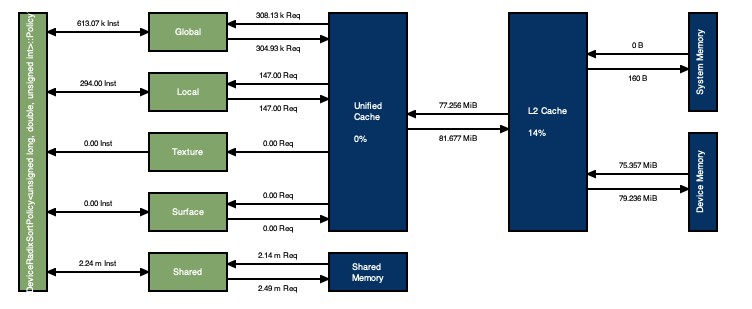
\includegraphics{attachments/louvain/Louvain_akamai.png}
\caption{Louvain\_akamai}
\end{figure}

It's clear that the bottleneck is at the device memory: most data are
read-once and write-once, no much possibility to reuse the data. The
kernel achieved 691 GB/s bandwidth utilization, \textasciitilde{}77\% of
the 32GB HBM2's 900 GB/s capability. This high bandwidth utilization
fits the memory access pattern: mostly regular and coalesced. The
particular issue here is not the kernel implementation itself, it's the
usage of sorting: fully sorting the whole edge list maybe overkill.

One possible improvement is to use a custom hash table on the GPU, to
replace the sort + segmented reduce part. The hash table can also cut
the memory requirement by about 50\%.

\section{Next Steps}\label{next-steps-1}

\subsection{Alternate approaches}\label{alternate-approaches-1}

** Things tried but not really work **

Segmented sort and CUB segmented reduce: the original idea for
modularity optimization is to use CUB's segmented sort and segmented
reduce within each vertex's neighborhood to get the vertex-community
weights. However, CUB uses one block per each segment in these two
routines, and that creates huge load unbalance, as the neighbor list
length can have large differences. The solution is 1) use
vertex-community pairs as keys, and CUB's unsegmented sort; 2) implement
a load balanced segmented reduce kernel. This solution reduces the
sort-reduce time by a few X, and can be enabled by
\texttt{-\/-unify-segments} flag in the command line.

STL hash table on CPU: the std::map class has some performance issue
when used in multi-threading environment, and yields poor scalability;
it might be caused by using locks in the STL. The solution is to use a
size \textbar{}V\textbar{} array per thread for the vertices that thread
processes. Since within a thread, vertices are processed one by one, and
the maximum number of communities is \textbar{}V\textbar{}, so instead
of hash table, a flat size \textbar{}V\textbar{} array can replace the
hash table. This solution significantly reduces the running time, even
using a single thread. The multi-thread scalability is also much better.

Vanilla hash table on GPU: this can't be used, as keys (vertex-community
or community-community pair) and the values (edge weights) are both
64-bit, and there is currently no support of atomic-compare-and-exchange
operations for 128-bit data. Even if that's available, a vanilla table
only provides insert and query operations, but not accumulation of
values for the same key.

** Custom hash table **

Hash table can be used to accumulate the vertex to community weights
during modularity optimization iterations, and to get the community to
community edge weights during the graph contraction part of the
algorithm. Pervious implementations use hash tables as a common
practice. However, as mentioned above, vanilla hash tables storing
key-value pairs is not a good choice for Louvain.

Because Louvain not only needs to store the key-value pairs, it also
needs to accumulate the values associated with the same key: let the key
be the same vertex-community pair for modularity optimization, or the
same community-community pair for graph contraction. Ideally, if the
hash table provides the following functionalities, it would be much more
suitable for Louvain:

\begin{itemize}
\itemsep1pt\parskip0pt\parsep0pt
\item
  Only insert the key, in the first phase of using the hash table.
\item
  In the next phase, query the \textbf{positions} of the keys, and use
  atomic function to accumulate the values belonging to the same key, in
  a separate array.
\item
  There is a barrier between the two phases, all insertions of the first
  phase need to be visible to the second phase.
\end{itemize}

This kind of hash table removes the strong restriction that the
key-value pair needs to be able to handle by an atomic compare and
exchange operation, which imposed by vanilla hash table implementations.
The custom hash table is also more value accumulation friendly. It
replaces the sort-segmented reduce part, and can reduces the workload
from about O(6\textbar{}E\textbar{}) to O(2\textbar{}E\textbar{}), and
the memory requirement from 48\textbar{}E\textbar{} bytes to
24\textbar{}E\textbar{}. However, the memory access pattern now become
irregular and uncoalesced, it's still unknown whether it can actually
give performance gain.

\subsection{Gunrock implications}\label{gunrock-implications-1}

The core of Louvain implementation mainly uses: all-edges advance, sort,
segmented reduce, and for loops. The sort-segmented reduce operation is
actually a segmented keyed reduce; if that's a common operation shows up
in more algorithms, it could be made into a new operator. The all-edges
advance is used quite often in several applications, so warping it with
a simpler operator interface can be helpful.

\subsection{Notes on multi-GPU
parallelization}\label{notes-on-multi-gpu-parallelization-1}

When parallelizing across multiple GPUs, the community assignment of
local vertices and their neighbors need to available locally, either
explicitly by moving them using communication functions, or implicitly
by peer memory access or unify virtual memory. The communication volume
is in the order of O(\textbar{}V\textbar{}) and the computation workload
is at least in O(\textbar{}E\textbar{}), so the scalability should be
manageable.

When the number of GPUs is small, 1D partitioning can be used to divide
the edges, and replicate the vertices; so there is no need to do vertex
id conversion across multiple GPUs. When the number of GPUs is large,
the high-low degree vertex separation and partitioning scheme can be
used: edges are still distributed across GPUs, high degree vertices are
duplicated, and low degree vertices are owned by one GPU each. The
boundary to use different partitioning scheme is still unclear, but it's
likely that 8 GPUs within a DGX-1 can still be considered as a small
number, and use the simple 1D partitioning.

\subsection{Notes on dynamic graphs}\label{notes-on-dynamic-graphs-1}

Louvain is not directly related to dynamic graph. But it should be able
to run on a dynamic graph, provided the way to access all the edges is
the same. Community assignment from the pervious graph can be used as a
good starting point, if the vertex Ids are consistent and the graph is
not dramatically changed.

\subsection{Notes on larger datasets}\label{notes-on-larger-datasets-1}

The bottleneck of memory usage of the current implementation is on the
edge pair-weight sort function: that makes up about half of the memory
usage. Replace sort-segmented reduce with custom hash table can
significantly lower the memory usage.

Louvain needs to go over the whole graph once in each modularity
optimization iteration. If the graph is larger than the combined GPU
memory space, which forces streaming of the graph in each modularity
optimization iteration, the performance bottleneck will be the CPU-GPU
bandwidth. That can be an order slower than when the graph can be fully
fit in GPU memory. Considering the OpenMP implementation is not that
slow, using that may well be faster than moving the graph multiple times
across the CPU-GPU bridge.

\subsection{Notes on other pieces of this
workload}\label{notes-on-other-pieces-of-this-workload-1}

All parts of Louvain are graph related, and fully implemented in
Gunrock.

\end{document}
